%%%%%%%%%%%%%%%%%%%%%%%%%%%%%%%%%%%%%%%%%%%%%%%%%%%%%%%%%%%%%%%%%%%%%%%%%%%%%%
\documentclass[aspectratio=169]{beamer}            % Generate slides
%\documentclass[handout]{beamer}   % Generate handouts (6 slides to 1 page)
%\documentclass[aspectratio=169]{beamer}  % Use widescreen 16:9 aspect ratio
    % Possible aspect ratios are 16:9, 16:10, 14:9, 5:4, 4:3 (default) and 3:2
    % (Remember to remove the colon)

\usetheme{UoB}
%\usetheme[compress]{UoB}     % Compress the margins
%\usetheme[nourl]{UoB}        % Remove the footer with the URL
%\usetheme[nowatermark]{UoB}  % Remove the watermark from the title page

% Generate handouts with notes (3 slides + 3 notes to 1 page)
%\mode<handout>{
%  \pgfpagesuselayout{3 on 1 with notes}[a4paper,border shrink=10mm]
%}

\usepackage{nomencl} % nomenclature generation via makeindex
	\makenomenclature
\usepackage{tikz}
\usetikzlibrary{matrix,chains,scopes,arrows,positioning,fit,
	decorations.pathmorphing,decorations.markings,shapes,calc}
\usepackage[binary-units = true]{siunitx}
\usepackage{subfig}

\everymath{\displaystyle}

\graphicspath{{./Figures/}}

%%%%%%%%%%%%%%%%%%%%%%%%%%%%%%%%%%%%%%%%%%%%%%%%%%%%%%%%%%%%%%%%%%%%%%%%%%%%%%
\title[Bio-Inspired Distributed Sensing]{Bio-Inspired Distributed Sensing for
	Improved Flight Control}
%\subtitle{Subtitle}
\author{Sergio A. Araujo-Estrada}
\institute{Research Associate \\
	Aerospace Engineering Department \\
	\href{mailto:s.araujoestrada@bristol.ac.uk}{s.araujoestrada@bristol.ac.uk}}
\date{Thursday, May 3}

%%%%%%%%%%%%%%%%%%%%%%%%%%%%%%%%%%%%%%%%%%%%%%%%%%%%%%%%%%%%%%%%%%%%%%%%%%%%%%
\begin{document}

\titlepage

%%%%%%%%%%%%%%%%%%%%%%%%%%%%%%%%%%%%%%%%%%%%%%%%%%%%%%%%%%%%%%%%%%%%%%%%%%%%%%
\begin{frame}{Overview}
	\tableofcontents
\end{frame}

%%%%%%%%%%%%%%%%%%%%%%%%%%%%%%%%%%%%%%%%%%%%%%%%%%%%%%%%%%%%
\section{Introduction}
\subsection{Motivation}
\begin{frame}{Motivation}
  Please explain why you chose to investigate this particular aspect of science, computing, or engineering.
	\begin{itemize}
		\item{Intrinsic nonlinear dynamics}
		\item{Classic control strategies limitations}
		\item{Limitations of inertial controls}
		\item{Gust alleviation}
		\item{Aeroelastic effects}
		\item{Additional\/'Hidden' information}
	\end{itemize}
\end{frame}

%%%%%%%%%%%%%%%%%%%%%%%%%%%%%%%%%%%%%%%%%%%%%%%%%%%%%%%%%%%%
\subsection{Previous Research}
\begin{frame}{Previous Research}

	Explain all of the previous research you’ve done about this issue/challenge\ldots

  \begin{block}{A block}
    What was the goal of your previous research? Be sure to explain how you found it and anyone who might have helped you!.
  \end{block}

\end{frame}

%%%%%%%%%%%%%%%%%%%%%%%%%%%%%%%%%%%%%%%%%%%%%%%%%%%%%%%%%%%%
\subsection{Research Problem}
\begin{frame}{The problem or challenge}
  Please explain the question or problem that you investigated.
	\begin{itemize}
		\item Measure, acquire and process flow and load information
		\item Utilise it for flight control
	\end{itemize}
\end{frame}

%%%%%%%%%%%%%%%%%%%%%%%%%%%%%%%%%%%%%%%%%%%%%%%%%%%%%%%%%%%%
\begin{frame}{The hypothesis (or prediction)}
  What do you think will happen?
	\begin{itemize}
		\item AoA, Windspeed aero loads compuation/prediction/estimation
		\item Characterisation of pressure, strain \& force signals as function of ${\alpha}$, V
			\& ${\delta_{ail}}$
		\item Acquisition of training/testing daat sets for ANN for ${\alpha}$, V \&
			${\delta_{ail}}$ prediction
		\item Identification of stall characteristic markers in pressure \& strain signals, e.g.
			frequency, variance
		\item Acquisition of pressure \& strain characteristic response to change in ${q}$
		\item Explore pressure \& strain response to conditions similar to perching manoeuvre\
		\item Emulation of pressure \& strain response to gusts
		\item Identify pressure \& strain response to varying ${q}$, i.e. ${\dot{q}}$
		\item Vibration of wing has been observed during and after stall. How does this affect
			pressure \& strain signals?
		\item Identify pressure \& strain response to varying ${\delta_{ail}}$, i.e.
						${\dot{\delta}_{ail}}$
	\end{itemize}
\end{frame}

%%%%%%%%%%%%%%%%%%%%%%%%%%%%%%%%%%%%%%%%%%%%%%%%%%%%%%%%%%%%
\section{Experimental Setup}
\begin{frame}{Experimental Setup}
  A wing model was instrumented with a distributed array of sensors. The main characteristics of the instrumentation are as follows:
	\begin{itemize}
		\item{chord-wise array of 30 pressure ports in two sections along the span}
		\item{span-wise array with 16 strain gauges}
		\item{data acquisition system using MCU, sampling \@ \SI{100}{\hertz}}
		\item{1-DOF pitch motion wind tunnel rig}
		\item{servo system for automated motion}
	\end{itemize}
\end{frame}

%%%%%%%%%%%%%%%%%%%%%%%%%%%%%%%%%%%%%%%%%%%%%%%%%%%%%%%%%%%%
\begin{frame}[plain]
  \begin{figure}[!htb]
		\centering
		% WingSensorDescription.tex

\tikzstyle{RectObject1}=[rectangle,draw=blue,rounded corners,line width=0.5mm,minimum width=3.0em,%
	minimum height=11em]
\tikzstyle{RectObject2}=[rectangle,draw=blue,rounded corners,line width=0.5mm,minimum width=2em,%
	minimum height=2em]
\tikzstyle{RectObject3}=[rectangle,draw=blue,rounded corners,line width=0.5mm,minimum width=3em,%
	minimum height=3em]
\tikzstyle{RectObject4}=[rectangle,draw=blue,rounded corners,line width=0.5mm,minimum width=3.0em,%
	minimum height=4.5em]
\tikzstyle{LabelObject}=[fill=white,rectangle,rounded corners,line width=0.5mm,%
	align=center]
\tikzstyle{ArrowObject}=[red,line width=1.0mm, -latex]

\resizebox{!}{0.4\textwidth}{
	\begin{tikzpicture}
		\node[anchor=south west,inner sep=0] (image) at (0,0)%
			%{\includegraphics[width=\textwidth]{WingSensorDescription.eps}};
			{\includegraphics[width=\textwidth]{WingInstrumentation.eps}};
		% Define scope with 'image' dimensions as reference
		\begin{scope}[x={(image.south east)},y={(image.north west)}]
			%\draw[help lines,xstep=.05,ystep=.05] (0,0) grid (1,1);
			%\foreach \x in {0,1,...,9} { \node [anchor=north] at (\x/10,0) {0.\x}; }
			%\foreach \y in {0,1,...,9} { \node [anchor=east] at (0,\y/10) {0.\y}; }
			
			\only<2>{
			% Pressure Elements
			\draw(0.330,0.475) node[RectObject1] (PressSensSecA) {};
			\draw(0.730,0.475) node[RectObject1] (PressSensSecB) {};
			% Pressure Labels
			\draw(0.54,0.2) node[LabelObject] (PressSensSecA_Label) {Pressure Port\\Inserts};
			% Pressure Arrows
			\draw[ArrowObject] (PressSensSecA_Label.north) -- (PressSensSecA.east);
			\draw[ArrowObject] (PressSensSecA_Label.north) -- (PressSensSecB.west);
			}
			
			\only<3>{
			% Strain Elements
			\draw(0.240,0.580) node[RectObject2] (StrainSens01) {};
			\draw(0.425,0.580) node[RectObject2] (StrainSens02) {};
			\draw(0.630,0.580) node[RectObject2] (StrainSens03) {};
			\draw(0.820,0.580) node[RectObject2] (StrainSens04) {};
			% Strain Labels
			\draw(0.54,0.2) node[LabelObject] (StrainSens01_Label) {Strain Gauge\\Arrays};
			% Strain Arrows
			\draw[ArrowObject] (StrainSens01_Label.west) -- (StrainSens01.south east);
			\draw[ArrowObject] (StrainSens01_Label.north) -- (StrainSens02.south);
			\draw[ArrowObject] (StrainSens01_Label.north) -- (StrainSens03.south);
			\draw[ArrowObject] (StrainSens01_Label.east) -- (StrainSens04.south west);
			}
			
			\only<4>{
			% Servo Elements
			\draw(0.160,0.475) node[RectObject3] (Servo01) {};
			\draw(0.530,0.475) node[RectObject3] (Servo02) {};
			% Servo Labels
			\draw(0.340,0.2) node[LabelObject] (Servo_Label) {Control Surface\\Servos};
			% Servo Arrows
			\draw[ArrowObject] (Servo_Label.north) -- (Servo01.east);
			\draw[ArrowObject] (Servo_Label.north) -- (Servo02.west);
			}
			
			\only<5>{
			% Servo Elements
			\draw(0.130,0.815) node[RectObject4] (Pitot) {};
			% Servo Labels
			\draw(0.50,0.85) node[LabelObject] (Pitot_Label) {Auxiliary\\Pitot Tube};
			% Servo Arrows
			\draw[ArrowObject] (Pitot_Label.west) -- (Pitot.east);
			}
		\end{scope}
	\end{tikzpicture}
}
		\caption{Wing model experimental platform}
		\label{Fig:ExpPlatform}
	\end{figure}
\end{frame}

%%%%%%%%%%%%%%%%%%%%%%%%%%%%%%%%%%%%%%%%%%%%%%%%%%%%%%%%%%%%
\section{Experimental Results}
\begin{frame}[plain]{Experiment results}
  Record the information you get from your experiment.
	
	\begin{figure}[!htb]
		\centering
		\subfloat[Chord-wise Normalised Pressure\label{fig:ExpPlatform_Pressure}]{%
			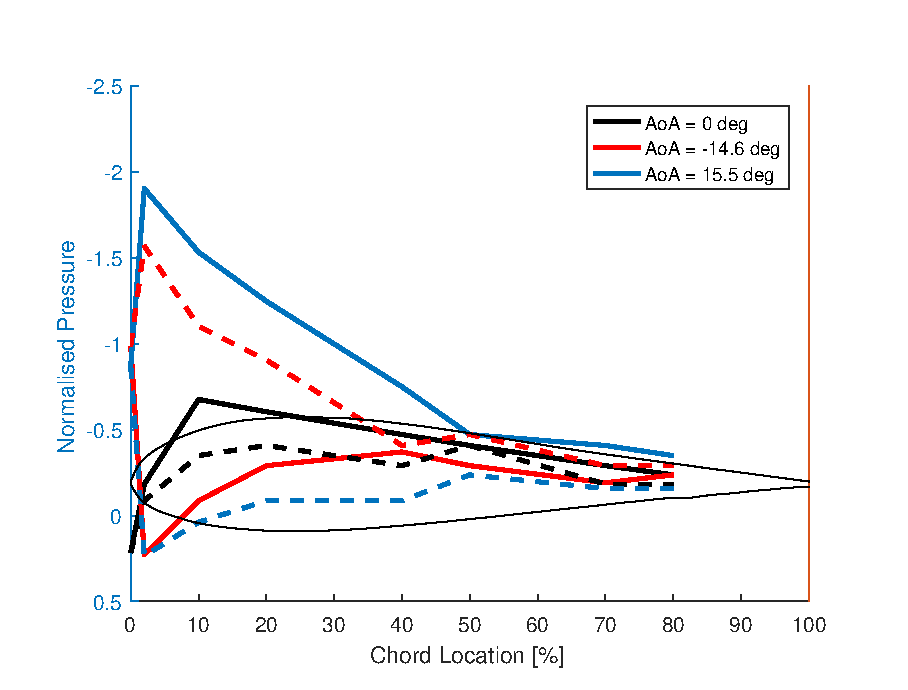
\includegraphics[width=0.4\textwidth]{PressureCoeffDistribution.eps}}\qquad
		\subfloat[Span-wise Normalised Bending Moment\label{fig:CharSignals_Bending}]{%
			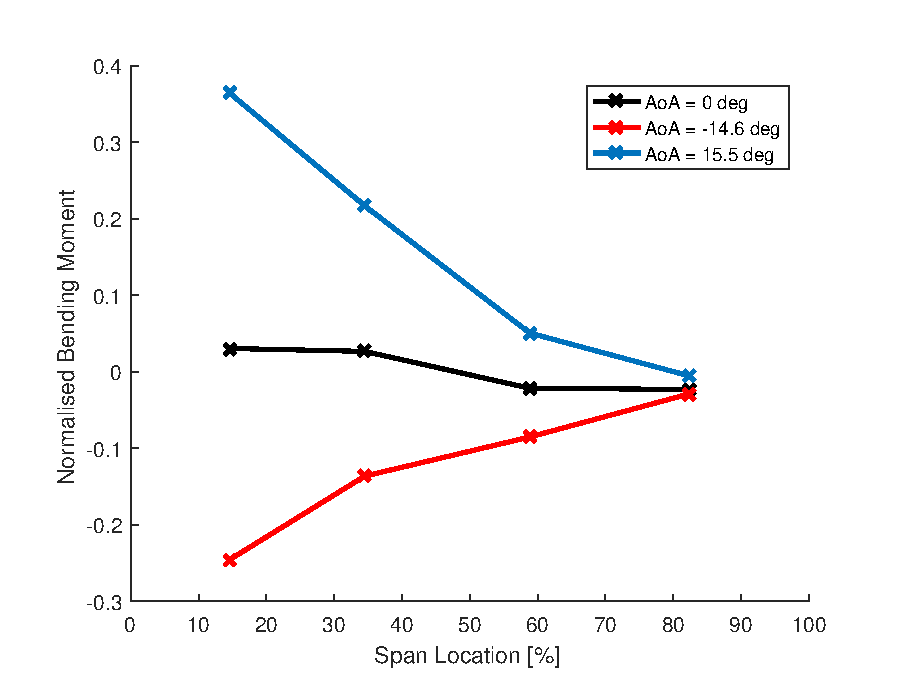
\includegraphics[width=0.4\textwidth]{BendingMomentDistribution.eps}}
		\caption{Characteristic signals from distributed sensing array}
		\label{Fig:CharSignals}
	\end{figure}

\end{frame}

%%%%%%%%%%%%%%%%%%%%%%%%%%%%%%%%%%%%%%%%%%%%%%%%%%%%%%%%%%%%
\begin{frame}{My discoveries}
	What did you learn after testing?
  \begin{itemize}[<+->]
  \item These will get revealed one by one
    \begin{itemize}
    \item Indented bullets
    \item Some more indented bullets
    \end{itemize}
  \item Another bullet point
  \item Yet another bullet point
  \end{itemize}
\end{frame}

%%%%%%%%%%%%%%%%%%%%%%%%%%%%%%%%%%%%%%%%%%%%%%%%%%%%%%%%%%%%
\begin{frame}[plain]
  This is the most important takeaway that everyone has to remember.
\end{frame}

%%%%%%%%%%%%%%%%%%%%%%%%%%%%%%%%%%%%%%%%%%%%%%%%%%%%%%%%%%%%
\section{Conclusions}
\begin{frame}{Conclusions}
	What is the conclusion of your experiment?
	Did the results support your hypothesis or predicted outcome?
	How will your findings help the area of science you’ve researched?
\end{frame}

%%%%%%%%%%%%%%%%%%%%%%%%%%%%%%%%%%%%%%%%%%%%%%%%%%%%%%%%%%%%
\section{Further Work}
\begin{frame}{Further Work}
	What will you do with your findings next?
	How will you further your research/findings?
\end{frame}

%%%%%%%%%%%%%%%%%%%%%%%%%%%%%%%%%%%%%%%%%%%%%%%%%%%%%%%%%%%%
\end{document}

%%%%%%%%%%%%%%%%%%%%%%%%%%%%%%%%%%%%%%%%%%%%%%%%%%%%%%%%%%%%%%%%%%%%%%%%%%%%%%
